\documentclass{article}
\usepackage{graphicx} % Required for inserting images
\usepackage{float}
\usepackage[T1]{fontenc}
\usepackage{amsmath}
\usepackage[margin=1in]{geometry}
\usepackage{booktabs}
\usepackage{tabularx}
\usepackage[hidelinks]{hyperref}

\title{Opening new puts only on Fridays, on the stress-sized put book}
\author{Experiment report \textperiodcentered{} L/S Gamma Desk, QUANTT}
\date{2026-11-02}

\begin{document}

\maketitle

\textbf{Question:} On the 35\% stress-sized \texttt{hedged} book, does allowing new puts only on Fridays earn more net P\&L than re-entering on any day? Under the Friday rule, a book closed midweek by its profit-take or stop waits for Friday to re-enter.

\textbf{Method:}

\begin{itemize}

\item \textbf{Pre-registered backtest:} the hypothesis card was committed before any run (commit bc742fd). The research switch was committed before it (73e16a4).

\item \textbf{Data:} the live paper rules (\texttt{configs/\allowbreak{}paper.\allowbreak{}toml}) are replayed on R2 replay snapshots v1 (config\_hash b040760187f0) over the development window 2014-06-02 to 2024-12-31. The hold-out (2025-01-01 to 2026-07-10) was not used.

\item \textbf{Book (every variant and the reference):} the \texttt{hedged} book of \texttt{2026-\allowbreak{}10-\allowbreak{}22-\allowbreak{}stress-\allowbreak{}sized-\allowbreak{}puts}.

\begin{itemize}

\item An always-on short 25-delta put, with the signal ignored and the flat exit off.

\item Sized at entry so that a one-day 20\% SPY drop, with IV at max(60\%, the put's IV), costs at most 35\% of \$250k (\$87,500).

\item A 10-share daily hedge.

\item The 1x-credit stop, the 50\% profit-take, the 7-DTE time exit and the 1-day cool-off.

\end{itemize}

\item \textbf{Variants:}

\begin{itemize}

\item \texttt{friday} (primary): \texttt{[backtest] entry\_\allowbreak{}weekdays = [4]}, a new research switch. New puts open only on Fridays; exits, stops and hedges are unchanged.

\item \texttt{tuesday\_\allowbreak{}roll} (sensitivity): \texttt{[exit] exit\_\allowbreak{}dte = 3}. The expiring put is held through the weekend and rolled on the Tuesday of expiry week.

\end{itemize}

\item \textbf{Comparison:} the registered \texttt{2026-\allowbreak{}10-\allowbreak{}22-\allowbreak{}stress-\allowbreak{}sized-\allowbreak{}puts/\allowbreak{}hedged} runs at the same spread multiple, reused and not rerun. With the switch off, the engine reproduces their equity exactly.

\item \textbf{Runs and costs:} every variant was run at 1x and 2x spreads. Costs are \$0.65 per contract and \$0.005 per share, with a \$1 minimum per order. Decisions, exits and hedges run at 10:15 ET; decisions read a 15-minute-old chain, and fills price on trades in the 15 minutes after. Spot comes from put-call parity on the 30-minute snapshot grid.

\end{itemize}

\section{Result vs the pass bar}

Every check had to hold at 1x and 2x. P\&L is net of costs in USD for the whole sized book. ES is the mean of the worst 5\% of daily P\&L.

\begin{center}\small
\begin{tabularx}{\linewidth}{>{\raggedright\arraybackslash}X l l l l l}
\toprule
\textbf{Check (\texttt{friday} vs \texttt{hedged})} & \textbf{1x value} & \textbf{1x bar} & \textbf{2x value} & \textbf{2x bar} & \textbf{Result} \\
\midrule
Net P\&L, full window & \$111,315 & > \$121,482 & \$90,120 & > \$101,172 & fail \\
Net P\&L, 2014-06 to 2019-12 & \$53,677 & > \$49,132 & \$44,433 & > \$42,687 & pass \\
Net P\&L, 2020-01 to 2024-12 & \$57,638 & > \$72,350 & \$45,688 & > \$58,485 & fail \\
ES 5\% within 1.10x & \ensuremath{-}\$2,803 & \ensuremath{\geq} \ensuremath{-}\$3,317 & \ensuremath{-}\$2,897 & \ensuremath{\geq} \ensuremath{-}\$3,404 & pass \\
Max drawdown \ensuremath{\leq} \$87,500 & \$32,301 & \ensuremath{\leq} \$87,500 & \$38,232 & \ensuremath{\leq} \$87,500 & pass \\
Event floor: Mon-Thu profit or stop exits \ensuremath{\geq} 25 & 28 & \ensuremath{\geq} 25 &  &  & met \\
\bottomrule
\end{tabularx}
\end{center}

\textbf{Verdict: failed.}

\begin{itemize}

\item Waiting for Friday cost about \$10k of net P\&L over 2014-2024 at both spreads. The loss is all in 2020-2024; 2014-2019 improved slightly.

\item The Friday book still makes money: +\$111k at 1x and +\$90k at 2x.

\item Its drawdown was less than half the reference's, but that comes from one path through March 2020, analysed below.

\end{itemize}

\subsection{Full-window numbers (not part of the bar)}

\begin{center}\small
\begin{tabularx}{\linewidth}{>{\raggedright\arraybackslash}X >{\raggedright\arraybackslash}X >{\raggedright\arraybackslash}X >{\raggedright\arraybackslash}X >{\raggedright\arraybackslash}X >{\raggedright\arraybackslash}X >{\raggedright\arraybackslash}X}
\toprule
\textbf{} & \textbf{hedged 1x} & \textbf{friday 1x} & \textbf{tuesday\_roll 1x} & \textbf{hedged 2x} & \textbf{friday 2x} & \textbf{tuesday\_roll 2x} \\
\midrule
Net P\&L & \$121,482 & \$111,315 & \$130,874 & \$101,172 & \$90,120 & \$111,414 \\
Sharpe & 0.52 & 0.57 & 0.72 & 0.43 & 0.45 & 0.60 \\
Max drawdown & \$70,362 & \$32,301 & \$47,634 & \$75,488 & \$38,232 & \$55,508 \\
ES 5\% (daily) & \ensuremath{-}\$3,016 & \ensuremath{-}\$2,803 & \ensuremath{-}\$2,573 & \ensuremath{-}\$3,094 & \ensuremath{-}\$2,897 & \ensuremath{-}\$2,689 \\
Round trips & 182 & 180 & 145 & 181 & 180 & 145 \\
Commissions (options /\allowbreak{} hedges) & \$5,955 /\allowbreak{} \$2,868 & \$5,846 /\allowbreak{} \$2,884 & \$4,716 /\allowbreak{} \$2,826 & \$5,918 /\allowbreak{} \$2,863 & \$5,846 /\allowbreak{} \$2,886 & \$4,728 /\allowbreak{} \$2,808 \\
\bottomrule
\end{tabularx}
\end{center}

\section{Charts}

\begin{figure}[H]\centering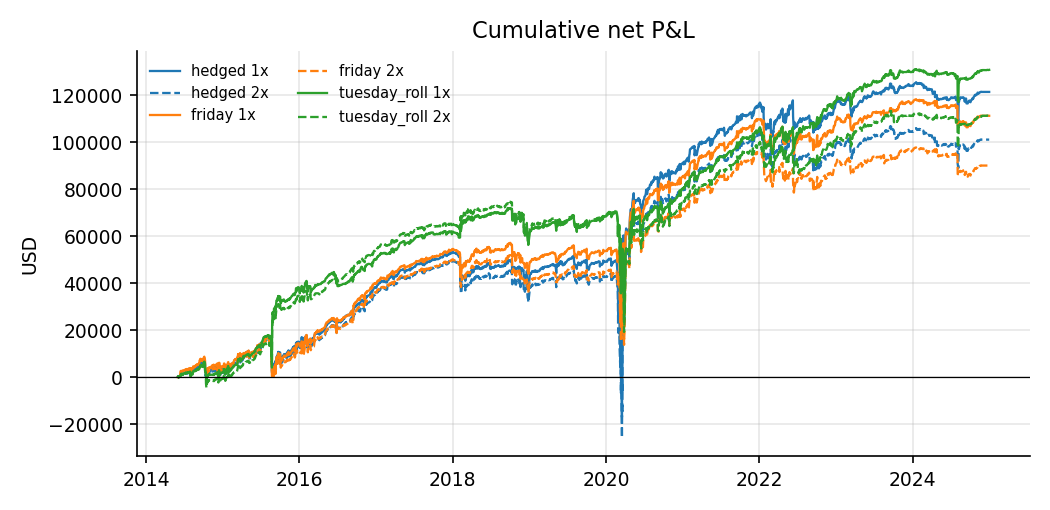
\includegraphics[width=0.92\linewidth]{figures/cum_pnl.png}\caption{Cumulative net P\&L, 1x solid and 2x dashed}\end{figure}

The three books track each other until 2020. \texttt{tuesday\_\allowbreak{}roll} pulls ahead in August 2015 and stays ahead to 2020. In March 2020 the reference falls furthest and then recovers most, \texttt{friday} falls and recovers less, and \texttt{tuesday\_\allowbreak{}roll} gives back its lead. From 2021, \texttt{friday} stays \$2k-13k below the reference.

\begin{figure}[H]\centering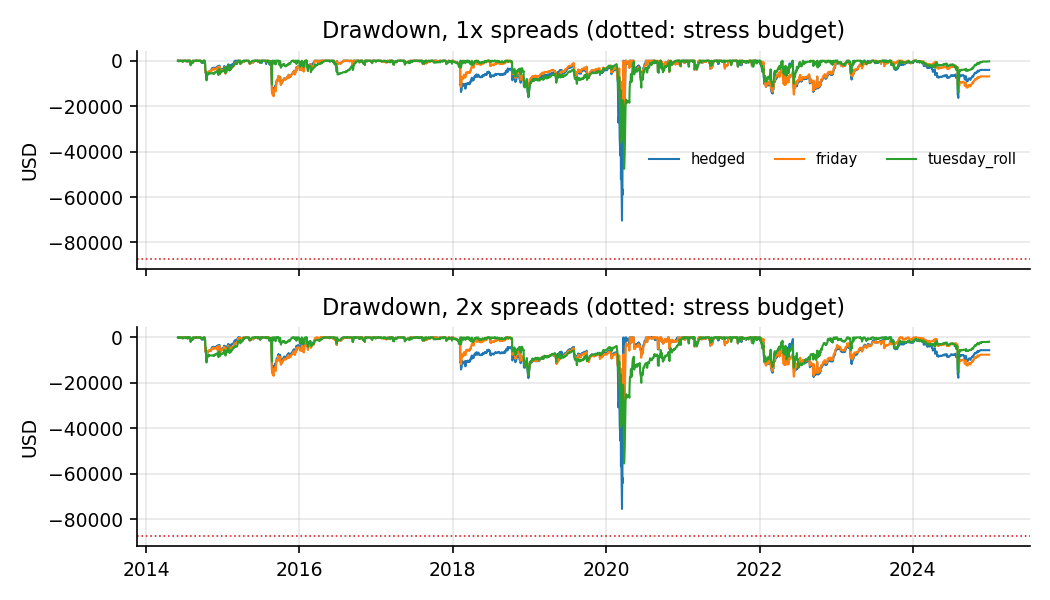
\includegraphics[width=0.92\linewidth]{figures/drawdown.png}\caption{Drawdown at 1x and 2x spreads}\end{figure}

Every book stays inside the \$87,500 stress budget (dotted). The deepest drawdown of every book is March 2020:

\begin{itemize}

\item reference: \$70k;

\item \texttt{friday}: \$32k;

\item \texttt{tuesday\_\allowbreak{}roll}: \$48k.

\end{itemize}

Outside March 2020 the three books' drawdowns are similar, mostly under \$20k.

\begin{figure}[H]\centering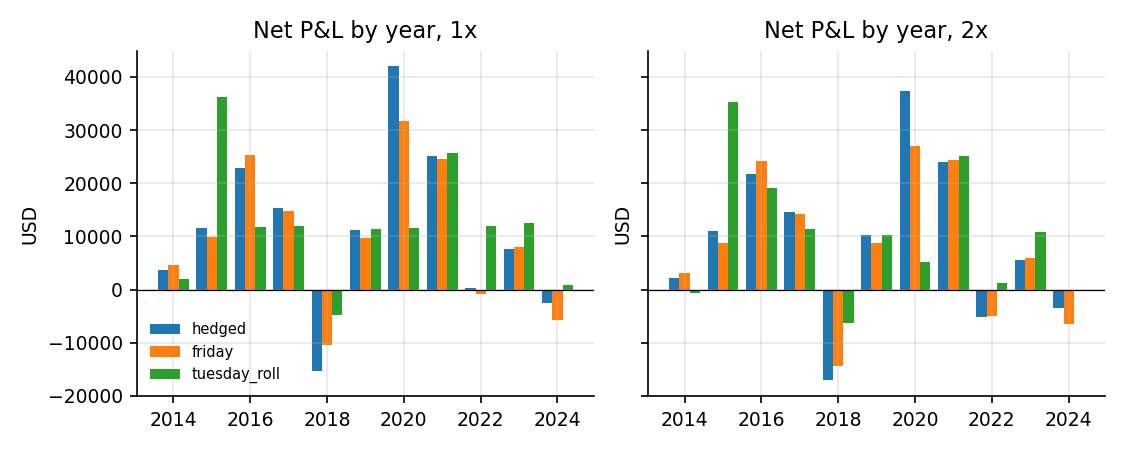
\includegraphics[width=0.92\linewidth]{figures/yearly.png}\caption{Net P\&L by year}\end{figure}

\texttt{friday}'s yearly results are close to the reference's in most years. The exceptions:

\begin{itemize}

\item 2020: \ensuremath{-}\$10.4k at 1x;

\item 2024: \ensuremath{-}\$3.1k;

\item 2018: +\$4.7k, when it lost less in the February volatility spike.

\end{itemize}

\texttt{tuesday\_\allowbreak{}roll} is far from the reference in several years: +\$24.7k in 2015 but \ensuremath{-}\$30.4k in 2020 at 1x.

\begin{figure}[H]\centering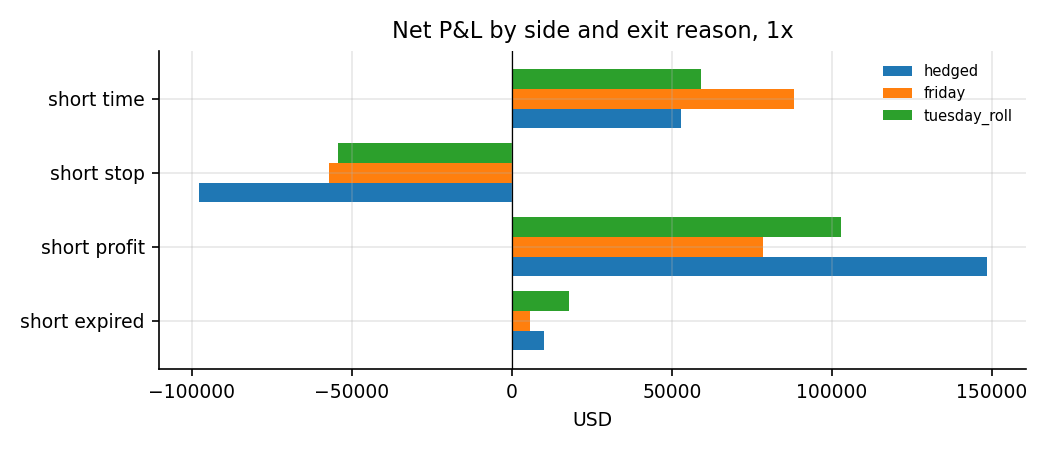
\includegraphics[width=0.92\linewidth]{figures/by_reason.png}\caption{Net P\&L by side and exit reason, 1x}\end{figure}

\texttt{friday} has fewer and smaller profit-takes and stops than the reference: 22 and 7 against 25 and 8. More of its P\&L arrives at the time exit. The swing comes mostly from March 2020, when the reference's 100-contract put was closed at its profit target and two earlier puts were stopped.

\begin{figure}[H]\centering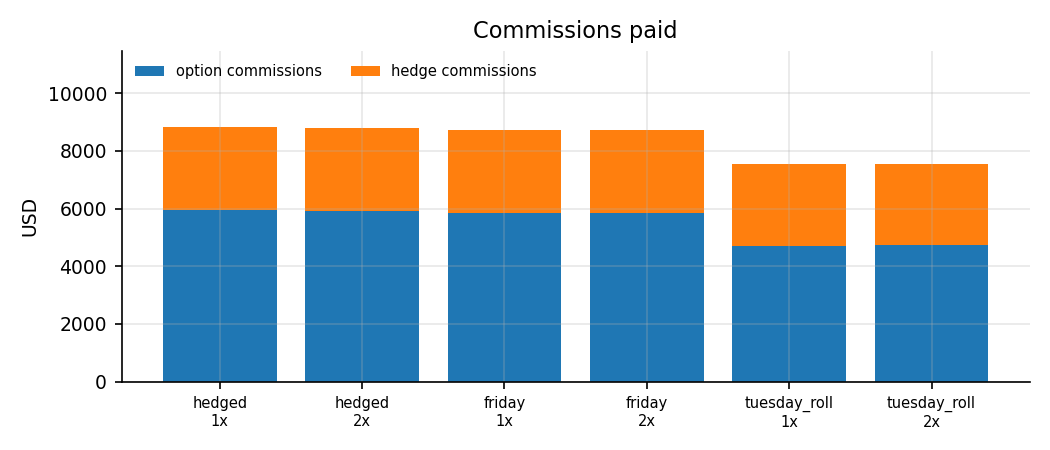
\includegraphics[width=0.92\linewidth]{figures/fees.png}\caption{Commissions paid}\end{figure}

Commissions barely change. \texttt{friday} makes 180 round trips against 182; the cost of waiting is lost exposure, not fees. \texttt{tuesday\_\allowbreak{}roll} pays about \$1,200 less in option commissions because its positions last longer (145 round trips).

\begin{figure}[H]\centering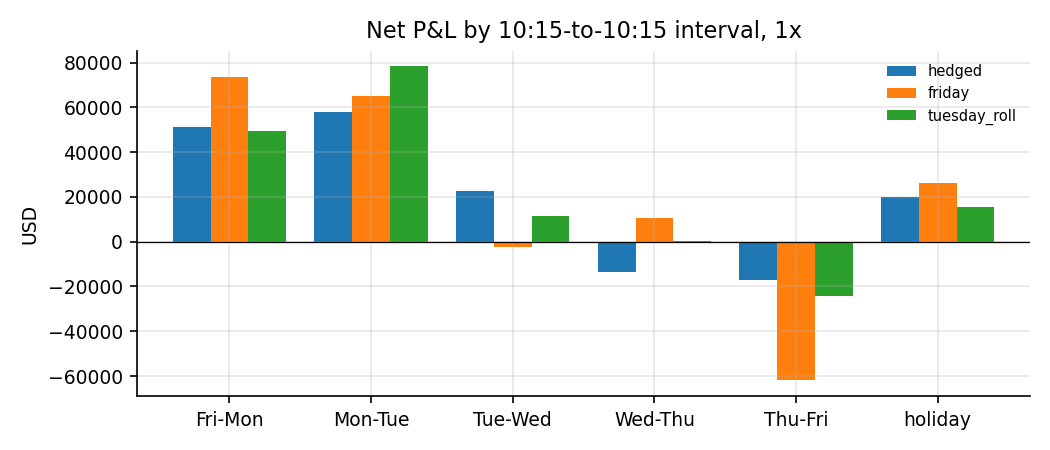
\includegraphics[width=0.92\linewidth]{figures/intervals.png}\caption{Net P\&L by 10:15-to-10:15 interval, 1x}\end{figure}

\texttt{friday} earns more over Friday-to-Monday and Monday-to-Tuesday intervals than the reference: +\$73k and +\$65k against +\$51k and +\$58k. It loses much more from Thursday to Friday: \ensuremath{-}\$62k against \ensuremath{-}\$17k. That gap is almost all 2020: Thursday-to-Friday intervals that year made \ensuremath{-}\$7.3k in \texttt{friday} and +\$31.0k in the reference. Most of it is one interval, 19 to 20 March 2020: the reference's 100-contract put gained \$35.7k, while \texttt{friday}'s 46-contract put lost \$11.9k. In the other years the two books' Thursday-to-Friday totals differ by at most \$3.5k.

\section{Analysis}

\textbf{What the rule changed.} \texttt{friday} opened all 180 of its puts on Fridays. The reference opened 138 on Fridays and 44 on other days. 112 of \texttt{friday}'s 180 entry dates are also reference entry dates; the rest are shifted by a few days, which changes everything after. The rule blocked 149 midweek entry decisions, and the book was flat on 181 decision days against 33 for the reference. The 28 Monday-to-Thursday profit-takes or stops that started those waits meet the event floor of 25.

\textbf{March 2020 is one path, not a weekday effect.} In the reference, the put opened in mid-February was stopped on 25 February, and two more puts were stopped before 13 March. The book then sold 100 contracts on Friday 13 March and took a +\$70.7k profit on 24 March. In \texttt{friday}, the 25 February stop was followed by a 46-contract entry on Friday 28 February. That put was never stopped: its hedged P\&L stayed above the stop through the crash. It closed at the time exit on 20 March for a small gain, and the book then sold 93 contracts on Friday 20 March.

So \texttt{friday} avoided two stops but missed most of the rally that the reference's 100-contract put caught. From 15 February to 30 April 2020 it made \$15.7k against \$21.6k at 1x. That one path explains its smaller drawdown. It is mechanical in the sense that the rule moved the entry dates, but which book wins depends on where the stops landed in a single crash, so it should not be read as a property of Friday entry.

\textbf{Outside March 2020 the rule still loses a little.} Excluding 15 February to 30 April 2020:

\begin{itemize}

\item \texttt{friday} made \$95.6k against \$99.9k at 1x, and \$77.8k against \$82.7k at 2x;

\item in 2020-2024 it trails by \$8.8k at 1x and \$6.7k at 2x;

\item in 2014-2019 it leads by \$4.5k at 1x and \$1.7k at 2x.

\end{itemize}

These year-by-year differences are a few thousand dollars on 10-20 round trips a year, about the size of one or two trades, and change sign from year to year. The evidence is that waiting for Friday does not add P\&L. It is not strong evidence that it subtracts P\&L either.

\textbf{The weekend pattern does not convert into a rule.} Sitting flat midweek gives up the Tuesday-to-Thursday intervals, which the reference made about \$9k on in total. Those intervals are small but positive for the reference, so skipping them costs a little. \texttt{friday}'s larger Friday-to-Monday total (+\$22.0k more than the reference) is spread over most years; only \$10.1k of it is 2020. Its larger Thursday-to-Friday loss is mostly 2020, and its whole Monday-to-Tuesday edge is 2020 (+\$15.1k in 2020 against +\$7.2k overall).

\textbf{Sensitivity \texttt{tuesday\_\allowbreak{}roll} (cannot pass this card).} Holding the expiring put to the Tuesday of expiry week earned \$130.9k at 1x and \$111.4k at 2x, with a Sharpe of 0.72 and 0.60. Against the reference it was:

\begin{itemize}

\item higher over the full window and in 2014-2019 at both spreads;

\item lower in 2020-2024 at both: \$62.4k against \$72.3k at 1x, and \$42.4k against \$58.5k at 2x.

\end{itemize}

Its gain is concentrated in a few years: +\$24.7k in 2015 (most of it in August 2015), +\$11.7k in 2022 and +\$10.4k in 2018, against \ensuremath{-}\$30.4k in 2020 and \ensuremath{-}\$11.1k in 2016. The book also missed hedges more often near expiry: hedges were skipped for missing deltas 35 times against 15 for the reference (10 for \texttt{friday}), because 3-DTE puts often have no smile fit. As a sensitivity it is a lead for a separate card, not a result.

\section{Verdict}

\textbf{Failed} per the pre-registered bar. \texttt{friday} loses on full-window and 2020-2024 net P\&L at both spreads, and wins only 2014-2019. The ES guard and the drawdown limit hold.

Archive Friday-only entry. If the PM wants to pursue the \texttt{tuesday\_\allowbreak{}roll} lead, it needs its own card with its own bar. That card should split out March 2020 and check the near-expiry hedge gaps first.

\section{Caveats}

\begin{itemize}

\item \textbf{In-sample:}

\begin{itemize}

\item The idea came from the 2026-10-31 strategy research report's check on \texttt{always25} (2014-2024).

\item The book is the 2026-10-22 primary, chosen after its results.

\item Before pre-registration, the reference's P\&L by interval and its entries by weekday were seen while testing the report code.

\end{itemize}

\item \textbf{One crash drives the drawdown result.} March 2020 decides both the 2020 loss and the smaller drawdown, through the order of stops in a single path.

\item \textbf{Sized book:} 11 to 100 contracts per entry across the three books. Large March 2020 fills use the same spread model as small ones.

\item \textbf{Spread model:} fitted on about two weeks of calm 2026 live quotes; the 2x run is the stress test.

\item \textbf{Data gaps:}

\begin{itemize}

\item R2 has no month-end weekdays, so about 3.3\% of scheduled times are skipped (89 days).

\item \texttt{friday} had 5 unfilled orders and 10 missing deltas, against 31 and 35 for \texttt{tuesday\_\allowbreak{}roll}.

\end{itemize}

\item \textbf{Few events:} 28 Monday-to-Thursday profit or stop exits met the pre-registered floor of 25. But 7 were on Thursdays, and after 6 of those \texttt{friday} re-entered on the Friday, as the reference would have, so only about 22 exits caused a longer wait than the reference's.

\item \textbf{Holidays:} if Friday is a market holiday, \texttt{friday} waits a full week to re-enter.

\end{itemize}

\section{Trials}

4 trials for this experiment (2 variants \ensuremath{\times} 1x and 2x, one run of \texttt{experiment.\allowbreak{}py}; the registry tags it 954824c, the batch's last pre-registration commit, which contains this card's bc742fd), plus the baseline's 2. The reference \texttt{2026-\allowbreak{}10-\allowbreak{}22-\allowbreak{}stress-\allowbreak{}sized-\allowbreak{}puts/\allowbreak{}hedged} was reused, not rerun. Three other experiments from the same batch were run at the same time on the same branch. The pass bar was not changed.

\end{document}
